\begin{figure}[ht]
	\centering
    \tikzstyle{vertex}=[circle, fill=black!25, minimum size=10pt, inner sep=0pt]
    \tikzstyle{edge} = [draw, thick, -]
    \tikzstyle{selected edge} = [draw, line width=2pt,-,red!50]
    \begin{subfigure}{.15\linewidth}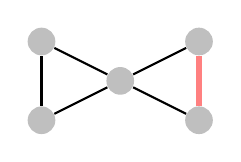
\begin{tikzpicture}[scale=1, auto, swap]
	    \foreach \pos/\name in {{(0,0)/1}, {(-1,-0.5)/2}, {(-1,0.5)/3}, {(1,-0.5)/4}, {(1,0.5)/5}}
	        \node[vertex] (\name) at \pos {};
	    \foreach \source/ \dest in {1/2, 2/3, 3/1, 1/4, 4/5, 1/5}
			\path[edge] (\source) -- (\dest);
		\path[selected edge] (4) -- (5);
	\end{tikzpicture}\end{subfigure}
    {\LARGE$+$}\hspace{0.5ex}
	\begin{subfigure}{.12\linewidth}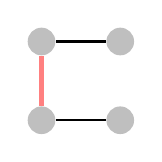
\begin{tikzpicture}[scale=1, auto, swap]
		\foreach \pos/\name in {{(1,-0.5)/4}, {(1,0.5)/5}, {(2,-0.5)/6}, {(2, 0.5)/7}}
			\node[vertex] (\name) at \pos {};
		\foreach \source/ \dest in {4/5, 4/6, 5/7}
			\path[edge] (\source) -- (\dest);
		\path[selected edge] (4) -- (5);
	\end{tikzpicture}\end{subfigure}
    {\LARGE$\rightarrow$}\hspace{0.5ex}
	\begin{subfigure}{.15\linewidth}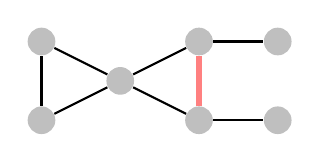
\begin{tikzpicture}[scale=1, auto, swap]
		\foreach \pos/\name in {{(0,0)/1}, {(-1,-0.5)/2}, {(-1,0.5)/3}, {(1,-0.5)/4}, {(1,0.5)/5}, {(2,-0.5)/6}, {(2, 0.5)/7}}
			\node[vertex] (\name) at \pos {};
		\foreach \source/ \dest in {1/2, 2/3, 3/1, 1/4, 4/5, 1/5, 5/7, 4/6}
			\path[edge] (\source) -- (\dest);
		\path[selected edge] (4) -- (5);
	\end{tikzpicture}\end{subfigure}
	\caption{A 2-clique sum of two graphs.}\label{fig:clique_sum}
\end{figure}
